%-----------------------------------------------------------------------------%
\chapter{\babEmpat}
%-----------------------------------------------------------------------------%

%-----------------------------------------------------------------------------%
\section{Implementasi Aplikasi}
%-----------------------------------------------------------------------------%

Implementasi aplikasi merupakan tahapan realisasi dari perancangan yang telah dibuat. Pada tahap ini akan dilakukan penjelasan mengenai antarmuka aplikasi “SiPJabS: Sistem Pengawakan Jabatan Struktural di Universitas Telkom”. 

\subsection{Implementasi Admin}

\begin{enumerate}
	
	\item Halaman Login Admin
	\begin{figure}
		\centering
		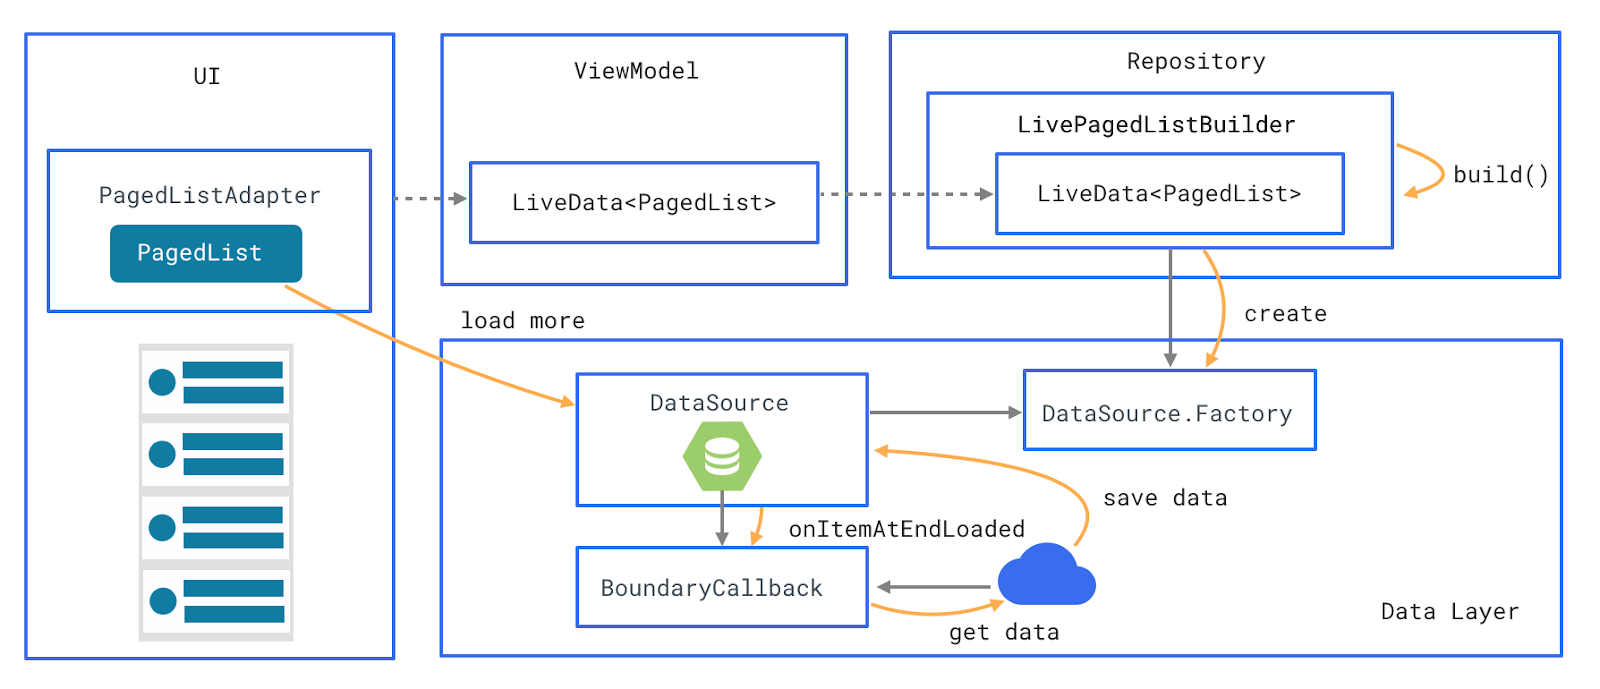
\includegraphics[width=0.9\textwidth]
		{pics/PagingLib.png}
		\caption{Paging Lib Android}
		\label{fig:CC10}
	\end{figure}

\end{enumerate}


\blindtext \\


%-----------------------------------------------------------------------------%
\section{Pengujian Aplikasi}
%-----------------------------------------------------------------------------%
\blindtext \\

\begin{figure}
	\centering
	\begin{tabular}[c]{cc}
		
		\begin{subfigure}[t]{0.45\textwidth}
			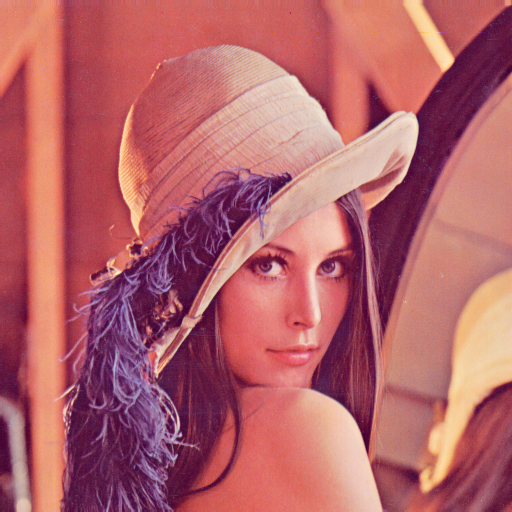
\includegraphics[width=\linewidth]{pics/lena.png}
			\caption{Testing With Lena} \label{fig:4a}
		\end{subfigure}
		\hspace*{\fill} % separation between the subfigures
		
		\begin{subfigure}[t]{0.45\textwidth}
			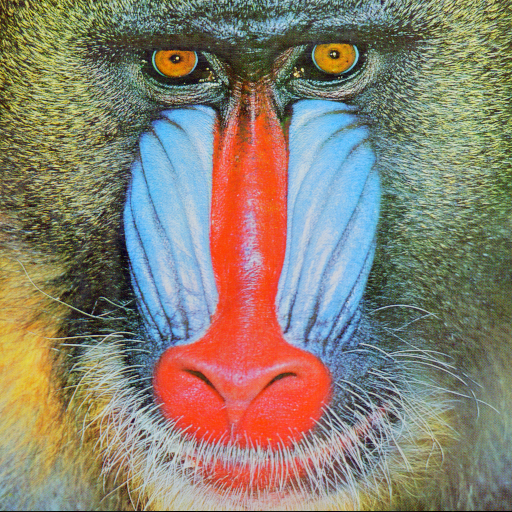
\includegraphics[width=\linewidth]{pics/baboon.png}
			\caption{Testing With Baboon} \label{fig:4b}
		\end{subfigure}
		
	\end{tabular}
	\caption{Pengujian Gambar Pada Aplikasi Z}
	\label{fig:41}
\end{figure}

%-----------------------------------------------------------------------------%
\subsection{Pengujian Alpha}
%-----------------------------------------------------------------------------%

\blindtext \\



\subsection{Pengujian Fungsionalitas}
\blindtext \\

\subsection{Pengujian Kesesuaian}
\blindtext \\

%-----------------------------------------------------------------------------%
\subsection{Pengujian Beta}
%-----------------------------------------------------------------------------%

\blindtext \\


%-----------------------------------------------------------------------------%
\section{Diskusi Hasil Pengujian}
%-----------------------------------------------------------------------------%

\begin{figure}
	\centering
	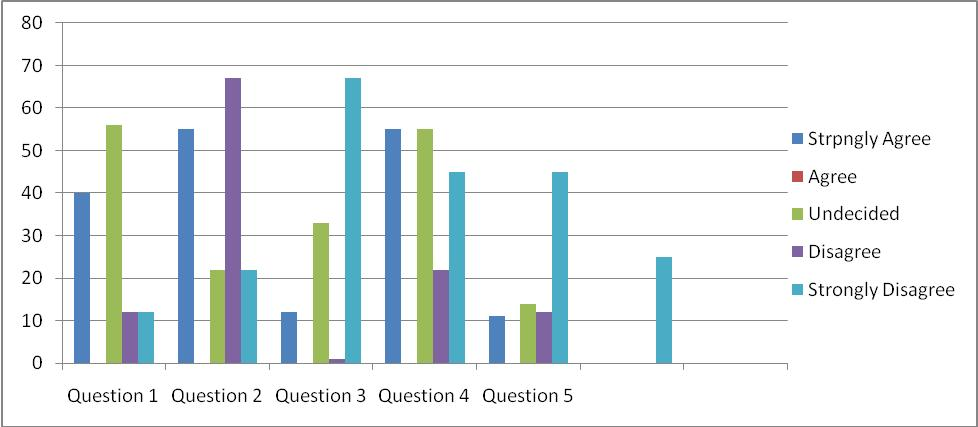
\includegraphics[width=0.8\textwidth]
	{pics/graph1.jpg}
	\caption{My Survey Results 2020}
	\label{fig:42}
\end{figure}

\blindtext \\